\section{Push relabel}
 
\begin{figure}[H]
 \centering 
	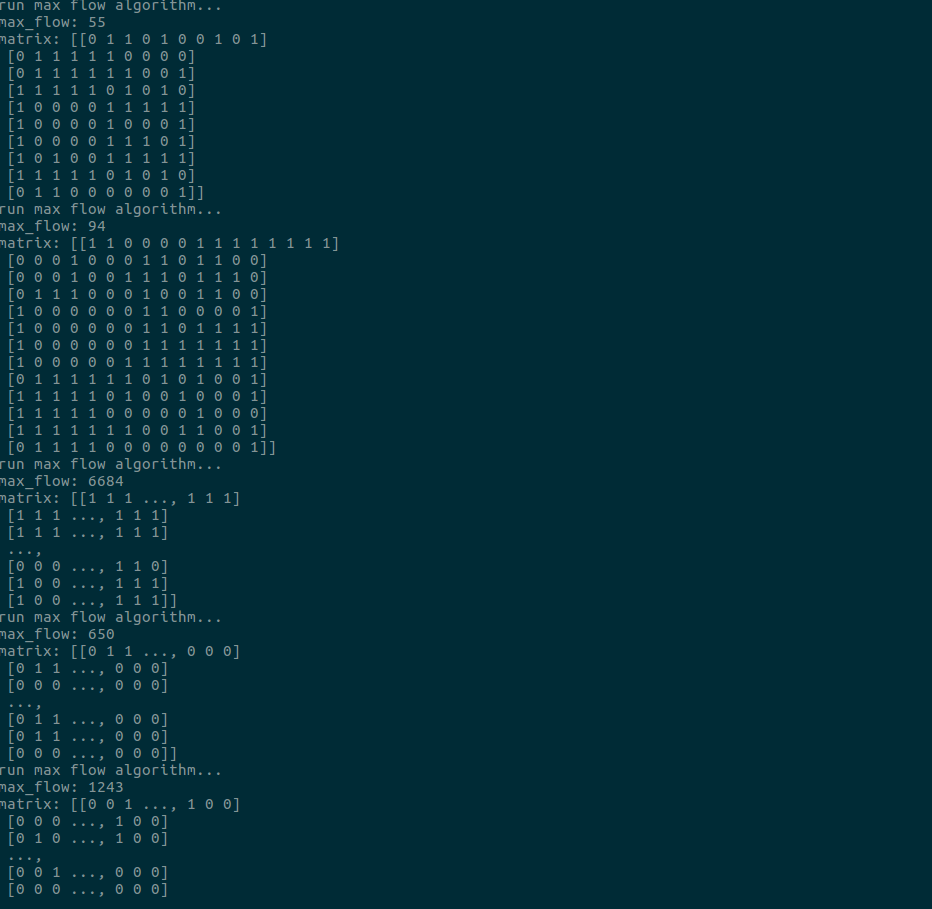
\includegraphics[width = 0.8\textwidth,height = 0.25\textheight]{work5/push1}
\end{figure} 	
the test result on `problem2.data' is showed above,
 the correctness of algorithm can be validated by broute fource.
 It is worth noting that using push relabel insead of Ford Fulkerson 
 is wise since time complexity.